\chapter{Objectives}

The goal of this project is the development and test of a low-cost electrical conductivity meter for liquids to be used as an aid to measure and analyze the flow in a photobioreactor.

This photobioreactor is used to grow algae that produce lipids from carbon dioxide via photosynthesis. These lipids can be processed to biofuel and other oil-derivatives, replacing crude oil as precursor. In order to be economical viable, the reactor has to feature minimal investment and operating cost.

To better develop, compare and optimize different reactor concepts, a computational fluid dynamics model is being developed. In order to validate this model, and to generate data to feed into it, the real flow conditions in an actual reactor have to be studied.

The scope of this work is the development and test of a sensor system to make that possible. The method chosen beforehand was to measure the fluids electrical conductivity, which can be changed easily by adding water with differing salt concentrations. Commercially available conductivity meters are built to measure with high accuracy in order to obtain information about a liquids absolute salinity and relatively expensive. Our use case however does not need to create high accuracy absolute measurements, but measure a relative change allowing to distinguish two different liquids by their salinity. However, this needs to happen very fast and at a lot of different points in the stream. The more positions measured, the more complete the picture of the flow becomes. Therefore, the cost per sensor has to be low, to not put a restraint on the total number of points that can be measured.

The actual flow analysis is not part of this work, but rather the creation of a tool to make it possible. As such, the system needs to be designed to be used by others, not the creator himself. This thesis therefore describes a product development process rather than a scientific study.

\section{Requirements}

The method to explore the flow conditions in the bioreactor used in this project is to measure the conductivity of the flowing water on multiple points with a high frequency. The conductivity is then changed by adding saltwater to the streaming freshwater, or by replacing the freshwater feed with a saltwater feed. The sensors then measure the increase in conductivity, signaling the arrival of the saltwater at certain positions. By mapping out the positions and the conductivity over time, an image of the flow can be generated. To get a usable image of the flow, the system has to meet certain requirements, which are described in this section.

\subsection{Spacial and Time Resolution}

The spacial and time resolution decide the granularity of the flow image.

The flow speed $ v $ of the stream is approximately \unitfrac[1]{m}{s}. This allows us to create a relation \ref{eq:res0} between the spacial resolution $ \diff s $ and the time resolution $ \diff t $.

\begin{equation}
	v = \dfrac{\diff s}{\diff t}
\label{eq:res0} 
\end{equation}

For example, a spacial resolution of \unit[1]{cm} would require a time resolution of \unit[0.01]{s}. However, this assumes the size $ l $ of the sensor and the time $ \tau $ a measurement takes to be infinitesimal small, while in reality it is not. To accommodate for that, factors $ n $ \ref{eq:resn} and $ k $ \ref{eq:resk} are introduced, describing the ratio of the resolutions to the actual sizes.

\begin{equation}
	n = \dfrac{l}{\diff s}
\label{eq:resn} 
\end{equation}

\begin{equation}
	k = \dfrac{ \tau}{\diff t}
\label{eq:resk}
\end{equation}

\begin{equation}
	v = \dfrac{\diff s}{\diff t} = \dfrac{k \cdot l}{n \cdot \tau}
\label{eq:res1} 
\end{equation}

Using $ 1 $ for $ n $ and $ 0.1 $ for $ k $ results in a sensor that has a size $ l $ of \unit[1]{cm}, and a $ \tau $ of \unit[1]{ms}. This ensures that the time for a measurement is only a tenth of the time it takes a control volume of fluid to flow over the sensors, as shown in \ref{fig:cv} , avoiding a smearing of the measurement over multiple control volumes.

\begin{figure}
	\begin{center}
		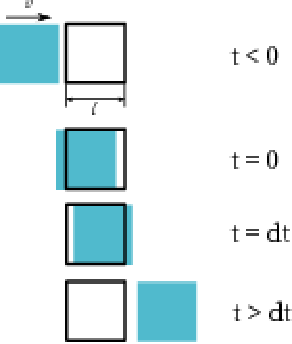
\includegraphics[width=0.45\textwidth]{images/resolution.pdf} 
		\caption{Control volume moving over sensor [redo in tikz]}
		\label{fig:cv}
	\end{center}
\end{figure}

\subsection{Electrical Conductivity Resolution}

To measure the arrival of the new water stream after switching the water feed, the system has to be able to distinguish between water with different salinity. The water used normally in the reactor is tap water with a salinity of about \unitfrac[5e-3]{S}{m}. The salinity of the added saltwater can be chosen freely. Sea water has a salinity of about \unitfrac[5]{S}{m} and offers a sensible choice. [sources for salinity]

\subsection{Cost}

The more sensors used, the more points in the stream can be measured and the better the image of the stream gets. Therefore, the cost per sensor has to be low enough to not be prohibitive of adding more sensors. [Why 10 bucks?]

\subsection{Usability}

The sensor system is meant to be used in the algae reactor in the algae lab at Airbus [insert correct name]. It has to be possible to easily mount and remove the system to and from the reactor without having to dismantle it.

The system also has to be easy to use, so it can be helpful to the researchers working on the reactor. It has to work reliably and act according to expectations of the users. The chance of handling errors that lead to loss of data has to be minimized. All operations have to be documented in a minimal set of written instructions, so the system can still be used even if the designer isn't available anymore.

\begin{table}
    \label{tab:req}

    \begin{center}
        \def\arraystretch{1.5}
        \arrayrulecolor[HTML]{FAFAFA}
        \arrayrulewidth=0.2em
        \begin{tabularx}{\textwidth}{l|X|l}

\rowcolor[HTML]{FAFAFA}
Nr. & Requirement & Verification \\
\rowcolor[HTML]{E1F5FE}
1 & The system shall have a time resolution of \unit[1]{ms}. & Test \\
\rowcolor[HTML]{FFF9C4}
2 & The system shall have a spacial resolution of \unit[1]{cm}. & Inspection \\
\rowcolor[HTML]{E1F5FE}
3 & The system shall cost less than \euro{10} per sensor.  & Analysis \\
\rowcolor[HTML]{FFF9C4}
4 & The system shall be deployable in the algae reactor. & Demonstr. \\
\rowcolor[HTML]{E1F5FE}
5 & The system shall be able to distinguish liquids with a conductivity of \unitfrac[5]{S}{m} and \unitfrac[5e-3]{S}{m}.  & Test \\
\rowcolor[HTML]{FFF9C4}
6 & The system shall be easy to use by anybody with only a minimal set of written instructions. & Test, Review \\

        \end{tabularx}
    \end{center}
    \caption{Requirements [nicely colored table vs. standard table?]}
\end{table}
